%Plantilla anteproyecto TFG
%Última modificación: 28 de mayo de 2021
\documentclass[12pt,oneside,a4paper]{article}
\usepackage[spanish]{babel}
\usepackage[utf8]{inputenc}
\usepackage{graphicx}
\usepackage{amsmath}
\usepackage{amssymb}
\usepackage{xcolor}
\usepackage{subfigure}
\usepackage{url}
\usepackage{float}
\linespread{1}
\setlength{\parskip}{1\baselineskip}
\parindent 1cm
\sloppy


%Opciones que debes descomentar mientras estemos revisando el anteproyecto
\usepackage{lineno}
\linenumbers


\usepackage[pagebackref=true,breaklinks=true,letterpaper=true,colorlinks,bookmarks=true]{hyperref}


%lista de palabras que Latex no parte bien
\hyphenation{pa-la-bras lis-ta}

\begin{document}

\thispagestyle{empty}

\begin{center}

\begin{large}
Grado en Ingeniería en Sistemas de Información\\
Escuela Politécnica Superior\\
\end{large}
\vspace{1cm}


\includegraphics[width=8cm]{figuras/logo-uah.pdf}

\textbf{ANTEPROYECTO}

\vspace{1cm}

\begin{large}\textbf{\textit{Innovación Tecnológica en la Evaluación Geriátrica: Automatización de Pruebas SPPB mediante Aplicación Móvil y Plataforma Web}}\end{large}

\vfill

Abril - 2024

\end{center}

\begin{flushright}
\textit{Autor - \textbf{F. Javier Redondo García}} \\
\textit{Tutor - \textbf{Sergio Caro Álvaro}} \\
\textit{Cotutor - \textbf{Ana Jiménez Martín}}
\end{flushright}

\newpage

\section{Introducción}

El envejecimiento fisiológico eleva la incidencia de enfermedades y éstas repercuten en aspectos funcionales, lo que favorece la incapacidad. Se pretende detectar el decaimiento físico en sus etapas más tempranas para intentar retrasar el estado de fragilidad. Para ello se utiliza el Test de evaluación del desempeño físico (SPPB) del adulto mayor como ayuda a la valoración geriátrica integral. \\
El objetivo del trabajo 'Innovación Tecnológica en la Evaluación Geriátrica: Automatización de Pruebas SPPB mediante Aplicación Móvil y Plataforma Web' es facilitar y agilizar la intervención médica con ayuda de una aplicación móvil con la que se realizarán las pruebas y una plataforma web sustentada en una base de datos para representar la información generada.


\subsection{Estado del arte}
Otros trabajos, referencias... (e.g. \cite{bibtex}).

\section{Objetivos y campos de aplicación}
Destaca los objetivos particulares, y también los campos de aplicación (haz una lista con las aplicaciones reales de tu trabajo).

\section{Descripción del trabajo}
¿Cómo lo voy a hacer?
\begin{figure}[H]
  \centering
  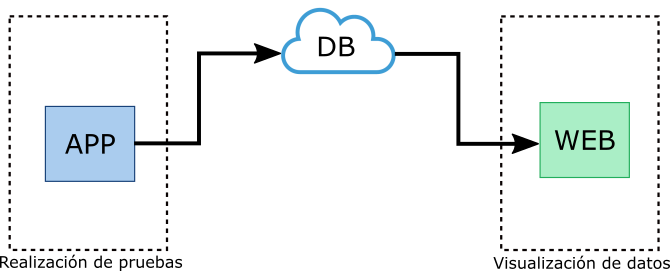
\includegraphics[width=15cm]{anteproyecto/figuras/tfg_diagramabloques_simple.png}
  \caption{Diagrama de bloques del funcionamiento básico del proyecto}
  \label{fig:ejemplo}
\end{figure}

\section{Fases de desarrollo}

\begin{enumerate}
\item Estudio de bibliografía y documentación sobre qué miden y cómo se realizan las pruebas SPPB.  Duración: 2 semanas.
\item Gestión de la base de datos en Firebase. Duración: 2 semanas
\item Desarrollo de la aplicación Android. Duración: 1 mes.
\item Desarrollo de la plataforma web. Duración: 1 mes.
\item Edición del documento final utilizando \LaTeX. Duración: 1 mes.
\end{enumerate}

\section{Medios disponibles}

\begin{itemize}
    \item Para la aplicación se hará uso de un teléfono móvil con sistema operativo Android versión 11 o superior. Este teléfono debe tener acceso a internet para poder comunicarse con la base de datos.
     El desarrollo Android se hará usando el entorno de desarrollo nativo Android Studio. \\
    \item Para la base de datos se utilizará Firebase Realtime Database, plataforma desarrollada por Google que ofrece un sistema NoSQL y sincronización automática entre los dispositivos de los usuarios en tiempo real. \\
    \item En cuanto a la web, se desarrollará con el lenguaje de programación Typescript, que trabaja sobre JavaScript y que permite añadir características estáticas de tipo, clases y módulos opcionales a JS. \\ 
    Como entorno de desarrollo se utilizará Angular, framework que ofrece un conjunto de herramientas completo y potente, que puede ser ideal para el objetivo del proyecto.
\end{itemize}






%Bibliografía
\bibliographystyle{plain}
\bibliography{bibliografia-tfc}


\end{document}
